\subsection{Application} %% TODO: another title...

\subsubsection{Class Diagram} %% TODO: another title...
See figure \vref{fig:uml}.\\
The class diagram shows the main classes of the model. Each variable of the class are detailled but only the main specific function that should be implemented are there and to avoid an overloading of the diagram we didn't list all the getters and setters of the variables. The hollow arrow shows the extended classes. For example, the classes Client and CoWorker extend User. The simple arrow shows a link between two classes and the indexes the number of this object that can be own by the class. When we see the link between address and user, it means that a user can have many addresses. But an organisation can have only one address.\\
Looking at the diagram we can see some classes extending user. There is client, coworker and moderator (extended by admin). This is due to the fact that there are all users but with specific rights on the website. Their is also the explicit link showing that a coworker of an organisation manage multiple client profiles. On another side, we have the moderator that are linked with the services categories. Another interesting part of the diagram is the architecture of the offer and demand. Each of these two objects are extending the "Service" abstract class and are linked with a transaction. The transaction is the conclusion of a matching. Service is an absctract class because we will never instantiate it directly.


\subsubsection{Sequences Diagrams} %% TODO: another title...

See figure \vref{fig:acceptService}.\\
See figure \vref{fig:addService}.\\
See figure \vref{fig:createUser}.\\
See figure \vref{fig:search}.\\
See figure \vref{fig:serviceFinished}.

\subsection{Physical Architectural View}



%– A physical architectural view of your software which describes how the logical architectural view is mapped to the physical components and connectors on your implementation platform (for example, different processors and other devices)
\begin{figure}[!ht]
	\begin{center}
		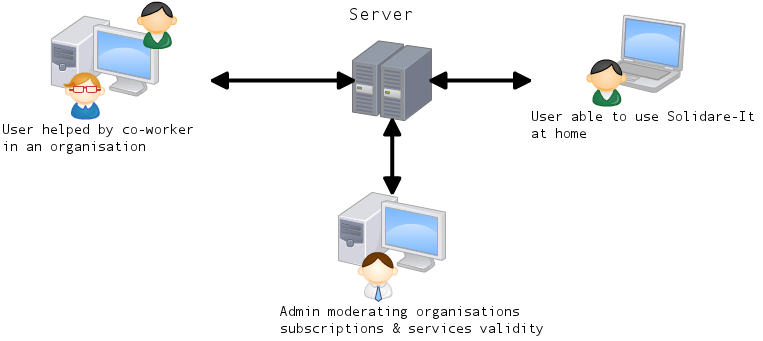
\includegraphics[width=\textwidth]{architectural_view_1.png}
		\caption{Website use}
		\label{fig:server}
	\end{center}
\end{figure}



\subsection{Pattern}
%– If applicable, a particular architectural style or pattern that is used. For example, it may be the case that the chosen web application framework imposes the use of a certain architectural pattern or architectural style (such as the model-view-controller architecture or MVC).

Ruby on Rails forces us to use the Model-View-Controller architectural style. Moreover, we all have experience with the MVC, then we will be more comfortable to code with this architecture.